\documentclass{article}
\usepackage[utf8]{inputenc}
\usepackage{amsmath}
\usepackage{graphicx}
\graphicspath{ {./images/} }

\title{Tarea 03 de Circuitos Lineales I}
\author{Gabriel Gamboa Vargas}
\date{Octubre 2021}

\begin{document}

\maketitle
\section{Ejercicio 1}
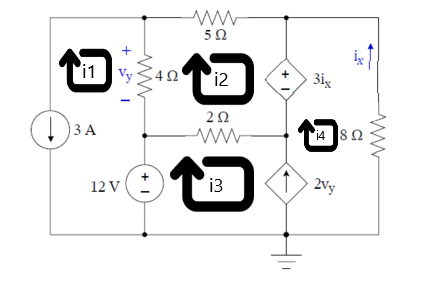
\includegraphics[]{images/ejercicio1.PNG}

\begin{equation} 
    i1 = -3A
\end{equation}
 
\begin{equation} 
    i4 = -ix
\end{equation}

\begin{equation} 
   {4\Omega} i1 - {4\Omega} i2 + {2\Omega}i3 +3i4 - {5\Omega}i2 = 0
\end{equation}
\\ \\
 Se usa un supernodo desde i3 hasta i4, donde hay una fuente de corriente.\\

\begin{equation}
   -12V + {2\Omega}i3 + 3i4 + {8\Omega}i4 = 0
\end{equation}
Con una limitación dada por la fuente de corriente: \\

\begin{equation}
   i3 + i2-i4 = -8(i1 -i2)
\end{equation}
\\ En forma matricial: \\ \\ 

$
\begin{pmatrix}
    1 & 0 & 0 & 0 \\
    4 & -9 & 2 & 3 \\
    0 & 0 & 2 & 11\\
    8 & -7 & 1 & -1
\end{pmatrix}
$$\begin{bmatrix}
    i1 \\
    i2 \\
    i3 \\
    i4 
\end{bmatrix}
$ = $\begin{bmatrix}
    -3 \\
    0 \\
    12  \\
    0
\end{bmatrix}
$ \\ \\ \\





\end{document}